\documentclass[a4paper,12pt,obeyspaces,spaces,hyphens]{article}

\def \trainingtitle{Linux debugging, profiling, tracing and performance analysis training}
\def \trainingduration{On-site training, 3 days}
\def \agendalanguage{english}
\def \training{debugging}

\usepackage{agenda}

\begin{document}

\feshowtitle

\feagendasummaryitem{Title}{
  {\bf \trainingtitle{}}
}
\feagendasummaryitem{Training objectives}{
  \begin{itemize}
    \vspace{-0.5cm}
  \item Be able to understand the main concepts of Linux that are
    relevant for performance analysis: process, threads, memory
    management, virtual memory, execution contexts, etc.
  \item Be able to analyze why a system is loaded and what are the
    elements that contributes to this load using common Linux
    observability tools.
  \item Be able to debug an userspace application using {\em gdb},
    either live or after a crash, and analyze the contents of ELF
    binaries.
  \item Be able to trace and profile a complete userspace application
    and its interactions with the Linux kernel in order to fix bugs
    using {\em strace}, {\em ltrace}, {\em perf} or {\em Callgrind}.
  \item Be able to understand classical memory issues and analyze them
    using {\em valgrind}, {\em libefence} or {\em Massif}.
  \item Be able to trace and profile the entire Linux system, using
    {\em perf}, {\em ftrace}, {\em kprobes}, {\em eBPF} tools, {\em
      kernelshark} or {\em LTTng}
  \item Be able to debug Linux kernel issues: debug kernel crashes
    live or post-mortem, analyze memory issues at the kernel level,
    analyze locking issues, use kernel-level debuggers.
    \vspace{-0.5cm}
  \end{itemize}
}
\feagendasummaryitem{Duration}{
  {\bf Three} days - 24 hours (8 hours per day).
}
\onsitepedagogics{40}{60}{debugging}
\feagendasummaryitem{Trainer}{
  Clément Léger
  \newline \url{https://bootlin.com/company/staff/clement-leger/}
}
\feagendasummaryitem{Language}{
  Oral lectures: English
  \newline Materials: English.
}
\feagendasummaryitem{Audience}{
  Companies and engineers interested in debugging, profiling and
  tracing Linux systems and applications, to analyze and address
  performance or latency problems.
}
\feagendasummaryitem{Prerequisites}{
  \begin{itemize}
    \prerequisitecommandline
    \prerequisiteembeddedlinux
    \prerequisiteenglish
  \end{itemize}
}
\ferequiredequipmentonsite{22.04}
\certificate{}
\disabilities{}

\feagendatwocolumn
{Hardware in practical labs}
{
  The hardware platform used for the practical labs of this training
  session is the {\bf STMicroelectronics STM32MP157D-DK1 Discovery
    board} board, which features:

  \begin{itemize}
  \item STM32MP157D (dual Cortex-A7) CPU from STMicroelectronics
  \item USB powered
  \item 512 MB DDR3L RAM
  \item Gigabit Ethernet port
  \item 4 USB 2.0 host ports
  \item 1 USB-C OTG port
  \item 1 Micro SD slot
  \item On-board ST-LINK/V2-1 debugger
  \item Arduino Uno v3-compatible headers
  \item Audio codec
  \item Misc: buttons, LEDs
  \end{itemize}
}
{}
{
  \begin{center}
  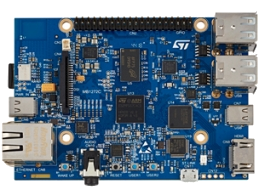
\includegraphics[width=5cm]{../slides/discovery-board-dk1/discovery-board-dk1.png}
  \end{center}
}

\section{Day 1 - Morning}

\feagendaonecolumn
{Lecture - Linux application stack}
{
  \begin{itemize}
  \item Global picture: understanding the general architecture of a
        Linux system, overview of the major components.
  \item What is the difference between a process and a thread, how
    applications run concurrently.
  \item ELF files and associated analysis tools.
  \item Userspace application memory layout (heap, stack, shared
    libraries mappings, etc).
  \item MMU and memory management: physical/virtual address spaces.
  \item Kernel context switching and scheduling
  \item Kernel execution contexts: kernel threads, workqueues,
    interrupt, threaded interrupts, softirq
  \end{itemize}
}

\feagendaonecolumn
{Lecture - Common analysis \& observability tools}
{
  \begin{itemize}
  \item Analyzing an ELF file with GNU binary utilities
    ({\em objdump}, {\em addr2line}).
  \item Tools to monitor a Linux system: processes, memory
    usage and mapping, resources.
  \item Using {\em vmstat}, {\em iostat}, {\em ps}, {\em top}, {\em
      iotop}, {\em free} and understanding the metrics they provide.
  \item Pseudo filesystems: {\em procfs}, {\em sysfs} and {\em
      debugfs}.
  \end{itemize}
}
\section{Day 1 - Afternoon}
\feagendaonecolumn
{Lab - Check what is running on a system and its load}
{
  \begin{itemize}
  \item Observe running processes using {\em ps} and {\em top}.
  \item Check memory allocation and mapping with {\em procfs} and {\em
      pmap}.
  \item Monitor other resources usage using {\em iostat}, {\em vmstat}
    and {\em netstat}.
  \end{itemize}
}

\feagendatwocolumn
{Lecture - Debugging an application}
{
  \begin{itemize}
  \item Using {\em gdb} on a live process.
  \item Understanding compiler optimizations impact on debuggability.
  \item Postmortem diagnostic using core files.
  \item Remote debugging with {\em gdbserver}.
  \item Extending {\em gdb} capabilities using python scripting
  \end{itemize}
}
{Lab - Solving an application crash}
{
  \begin{itemize}
  \item Analysis of compiled C code with compiler-explorer to understand
    optimizations.
  \item Managing {\em gdb} from the command line, then from an IDE.
  \item Using {\em gdb} Python scripting capabilities.
  \item Debugging a crashed application using a coredump with {\em gdb}.
  \end{itemize}
}

\section{Day 2 - Morning}

\feagendatwocolumn
{Lecture - Tracing an application}
{
  \begin{itemize}
  \item Tracing system calls with {\em strace}.
  \item Tracing library calls with {\em ltrace}.
  \end{itemize}
}
{Lab – Debugging application issues}
{
  \begin{itemize}
  \item Analyze dynamic library calls from an application using
    {\em ltrace}.
  \item Debug a misbehaving application using {\em strace}.
  \end{itemize}
}

\feagendatwocolumn
{Lecture - Memory issues}
{
  \begin{itemize}
  \item Usual memory issues: buffer overflow, segmentation fault,
    memory leaks, heap-stack collision.
  \item Memory corruption tooling, {\em valgrind}, {\em libefence},
    etc.
  \item Heap profiling using {\em Massif}
  \end{itemize}
}
{Lab – Debugging memory issues}
{
  \begin{itemize}
  \item Buffer overflow investigation with {\em libefence}.
  \item Memory leak and misbehavior detection with {\em valgrind} and
    {\em vgdb}.
  \item Performance issues due to memory over allocation.
  \item Visualizing application heap using {\em Massif}.
  \end{itemize}
}

\section{Day 2 - Afternoon}

\feagendatwocolumn
{Lecture – Application profiling}
{
  \begin{itemize}
  \item Performances issues.
  \item Gathering profiling data with {\em perf}.
  \item Analyzing an application callgraph using {\em Callgrind}
    and {\em KCachegrind}.
  \item Filtering the data set.
  \item Interpreting the data recorded by {\em perf}.
  \end{itemize}
}
{Lab - Application profiling}
{
  \begin{itemize}
  \item Profiling an application with {\em Callgrind}/{\em
      KCachegrind}.
  \item Analyzing application performances with {\em perf}.
  \item Generating a flamegraph using {\em FlameGraph}.
  \end{itemize}
}

\section{Day 3 - Morning}

\feagendatwocolumn
{Lecture - System wide profiling and tracing}
{
  \begin{itemize}
  \item System wide profiling using {\em perf}.
  \item Using {\em kprobes} to hook on kernel code without
    recompiling.
  \item {\em eBPF} tools ({\em bcctools}, {\em bpftrace}, etc) for
    complex tracing scenarios.
  \item Application and kernel tracing and visualization using {\em
      ftrace}, {\em kernelshark} or {\em LTTng}
  \end{itemize}
}
{Lab - System wide profiling and tracing}
{
  \begin{itemize}
  \item System profiling with {\em perf}.
  \item IRQ latencies using {\em ftrace}.
  \item Tracing and visualizing system activity using {\em
      kernelshark} or {\em LTTng}
  \end{itemize}
}

\section{Day 3 - Afternoon}

\feagendatwocolumn
{Lecture - Kernel debugging}
{
  \begin{itemize}
  \item Kernel compilation results (\code{vmlinux}, \code{System.map}).
  \item Understanding and configuring kernel {\em oops} behavior.
  \item Post mortem analysis using kernel crash dump with {\em crash}.
  \item Memory issues ({\em KASAN}, {\em UBSAN}, {\em Kmemleak}).
  \item Debugging the kernel using {\em KGDB} and {\em KDB}.
  \item Kernel locking debug configuration options (lockdep).
  \item Other kernel configuration options that are useful for debug.
  \end{itemize}
}
{Lab - Kernel debugging}
{
  \begin{itemize}
  \item Analyzing an {\em oops} after using a faulty module with
    {\em obdjump} and {\em addr2line}.
  \item Debugging a deadlock problem using {\em PROVE\_LOCKING} options.
  \item Detecting undefined behavior with {\em UBSAN} in kernel code.
  \item Find a module memory leak using {\em kmemleak}.
  \item Debugging a module with {\em KGDB}.
  \end{itemize}
}

\end{document}

